\documentclass{article}
\usepackage{tikz}
\usepackage{pgfplots}
\pgfplotsset{
    width = 17cm, height = 5cm,
    grid=major, minor y tick num=4,
    xlabel = {Time (s)}, ylabel = {Voltage (mV)},
    compat=1.18,
    every axis legend/.append style = {
        legend columns = 3,
        anchor = south east,
    },
	every axis title/.append style = {
		above, yshift=6pt,
	}
}
\usepackage{geometry}
\usepackage{siunitx}
\usepackage{amsmath}
	\geometry{top=1.0in, bottom=1.0in, left=1.0in, right=1.0in}
\usepackage{setspace}
	\onehalfspacing


\begin{document}

\begin{figure}[h]\centering
    \begin{tikzpicture}
        \begin{axis}[
            xmin=0, xmax=1.45,
            ymax=10,
            ytick distance=5
            ]
            \addplot+[no markers] table [ col sep=comma, x index=0, y index=1,]
            {variance.csv};
            \addlegendentry{Average}
            \addplot+[no markers, red] table [ col sep=comma, x index=0, y index=2,]
            {variance.csv};
        \addlegendentry{Maxima}
            \addplot+[no markers, red] table [ col sep=comma, x index=0, y index=3,]
            {variance.csv};
        \end{axis}
    \end{tikzpicture}

    \caption{Sampling rate: \SI{416}{\micro\second}. Data is indiscriminately decimated (for performance), then chunks of 10 are averaged. y-axis is shifted so lowest low is 0.}
\end{figure}

\begin{figure}[h]\centering
    \begin{tikzpicture}
        \begin{axis}[
            xmin=0, xmax=1.45,
            ymax=10,
            ytick distance=5
            ]
            \addplot+[no markers] table [ col sep=comma, x index=0, y index=1,]
            {mean_variance.csv};
            \addlegendentry{Average}
            \addplot+[no markers, red] table [ col sep=comma, x index=0, y index=2,]
            {mean_variance.csv};
        \addlegendentry{Maxima}
            \addplot+[no markers, red] table [ col sep=comma, x index=0, y index=3,]
            {mean_variance.csv};
        \end{axis}
    \end{tikzpicture}

    \caption{Same as above, but average over 5 recordings. Drift caused by inconsistent start of the experiment. Not helpful since the averaging is reducing the maxima.}
\end{figure}


\begin{figure}[h]\centering
    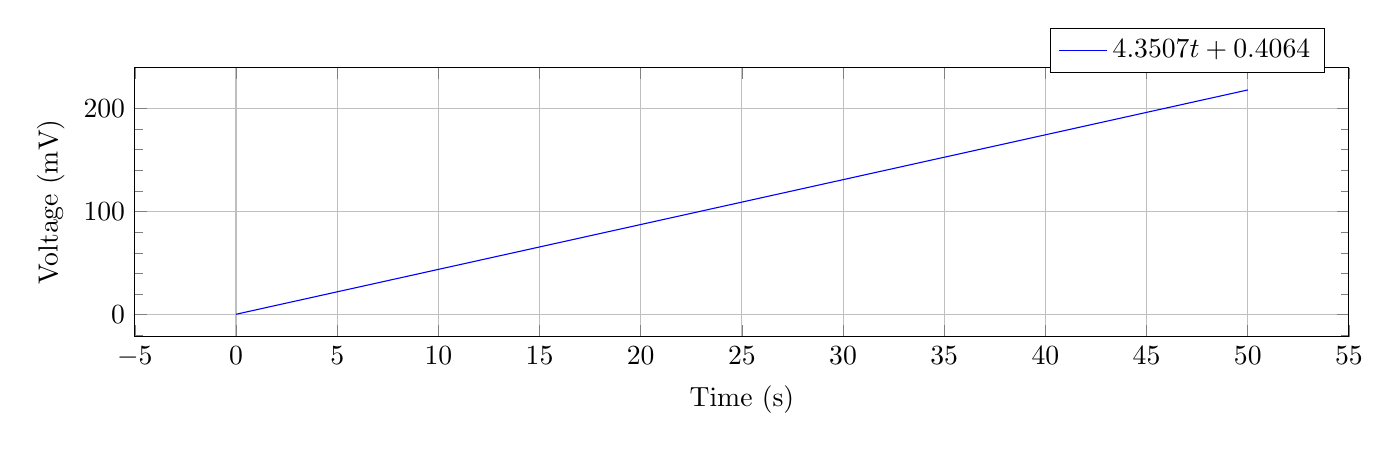
\begin{tikzpicture}
        \begin{axis}[domain=0:50, samples=100,]
            \addplot+ [no markers] {4.350656671570435*x+0.406389963452446};
            \addlegendentry{$4.3507t+0.4064$}
        \end{axis}
    \end{tikzpicture}
    \caption{Instron moving a rate of \SI{10}{\micro\metre\per\second} over \SI{50}{s} resulted in this motion.}
\end{figure}


\begin{equation*}
    \SI{10}{\micro\metre\per\second} \approx \SI{4.3507}{\milli\volt\per\second} \implies \SI{2.2985}{\micro\metre\per\milli\volt}
\end{equation*}

\end{document}
